%%%%%%%%%%%%%%%
%
% $Autor: Wings $
% $Datum: 2020-02-24 14:30:26Z $
% $Pfad: PythonPackages/Contents/General/PythonBarcode.tex $
% $Version: 1792 $
%
% !TeX encoding = utf8
% !TeX root = PythonPackages
% !TeX TXS-program:bibliography = txs:///bibtex
%
%
%%%%%%%%%%%%%%%





\chapter{Package \PYTHON{Python-Barcode}}

\section{Introduction}

The Python Barcode library is an open-source tool designed for generating barcodes in Python applications.Numerous barcode formats are supported by it, such as EAN-13, UPC-A, Code 39, and Code 128. These formats are frequently used in a variety of industries for logistical monitoring, inventory management, and product labeling. By offering a simple API that makes it easy for developers to generate barcodes, this library streamlines the barcode generating process. The Python Barcode library's flexibility is also seen in its support for PNG, SVG, and PDF output formats, which guarantee compatibility with a variety of operating systems and printing needs.

The Python Barcode library is notable for its highly customizable features. Barcodes can be made to look a certain way by developers by changing their size, adding textual annotations, and changing the font and color schemes. This is especially helpful for upholding industry standards and brand consistency. The library's smooth interface with other Python libraries, such PIL/Pillow for image editing, enables sophisticated customisation and easy incorporation into more extensive Python applications. Additionally, it allows batch processing, which makes it possible to generate many barcodes efficiently. This is crucial for large-scale manufacturing and retail operations\cite{Barrera:2020}.

The Python Barcode library is engineered to efficiently process large amounts of data in an efficient manner. To guarantee that only legitimate barcode data is handled, it has built-in validation and error-handling procedures, which lowers the possibility of errors and improves reliability. Because of this, it can be used in enterprise-level applications where speed and data integrity are essential. Because of its extensive feature set and user-friendly interface, the Python Barcode library is a valuable resource for developers wishing to integrate barcode generating into their Python projects. It offers a complete solution that can handle both simple and complex barcode generation requirements\cite{neubert:2023}.

\section{Barcodes}

\section{Description of Barcodes Used in Products and Foods}

Barcodes are a pervasive feature of contemporary retail and supply chain management, offering a uniform means of encoding product information. In Germany and the European Union (EU), barcodes play a pivotal role in facilitating efficient product identification, inventory management, and retail operations. This chapter examines the various types of barcodes in use, including an analysis of their components, encoding methods, technical features, and regulatory standards.

\begin{figure}[h]
	\centering
	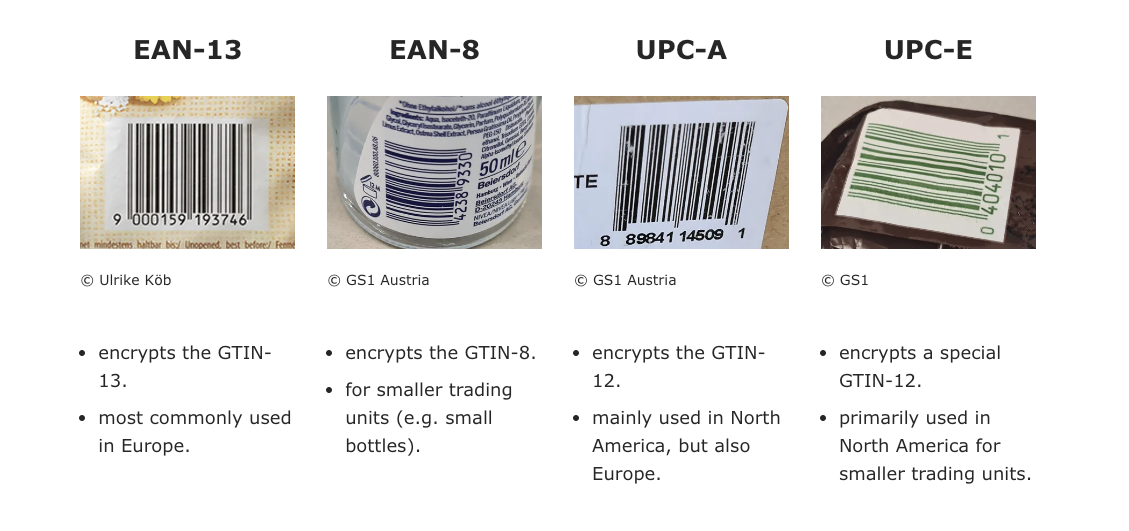
\includegraphics[width=0.8\textwidth]{barcode/barcodes.png}
	\caption{Examples of Barcodes}
	\label{fig:barcodes}
\end{figure}

\subsection{Types of Barcodes}

\subsubsection{UPC (Universal Product Code)}
UPC barcodes are a prevalent form of identification in North America, comprising 12 numeric digits. The UPC barcode is used to encode information such as the manufacturer and product identification number. Although less prevalent in Europe, some products exported to the EU may still bear UPC barcodes.

\subsubsection{Data Included}
The Universal Product Code (UPC) barcode is designed to encode a number of different pieces of information. These include the manufacturer's identification number, the product identification number, and a check digit used to detect errors \cite{eu_reg_1169_2011}.

\subsubsection{Technical Features}
\begin{itemize}
	\item \textbf{Numeric-only Encoding:} UPC barcodes consist only of numeric digits.
	\item \textbf{Fixed Length:} UPC barcodes are always 12 digits long.
\end{itemize}

\subsubsection{Example}
\begin{itemize}
	\item \textbf{UPC-A Barcode:} 036000291452
\end{itemize}

\subsubsection{EAN (European Article Number)}
EAN barcodes are the standard in Europe and consist of either 8 or 13 digits. The 13-digit EAN, also known as EAN-13, encodes the manufacturer and product identification number, along with a check digit for error detection. EAN-8 barcodes are used for smaller products where space is limited.

\subsubsection{Data Included}
The EAN-13 barcode encodes the manufacturer's country code, company prefix, item reference number, and a check digit \cite{ean_info}.

\subsubsection{Technical Features}
\begin{itemize}
	\item \textbf{Numeric-only Encoding:} EAN barcodes consist only of numeric digits.
	\item \textbf{Variable Length:} EAN-13 barcodes are 13 digits long, while EAN-8 barcodes are 8 digits long.
\end{itemize}

\subsubsection{Example}
\begin{itemize}
	\item \textbf{EAN-13 Barcode:} 4006381333931
\end{itemize}

\subsubsection{GS1 DataBar}
GS1 DataBar, formerly known as Reduced Space Symbology (RSS), is a family of barcode symbologies used for small items such as fresh foods and pharmaceuticals. It encodes various product attributes such as expiration date, weight, and serial numbers.

\subsubsection{Data Included}
GS1 DataBar can encode a variety of product attributes, including expiration date, weight, lot number, and serial number \cite{gs1_databar_info}.

\subsubsection{Technical Features}
\begin{itemize}
	\item \textbf{Variable Length:} GS1 DataBar can vary in length depending on the encoded data.
	\item \textbf{Alphanumeric Encoding:} GS1 DataBar can encode both numeric and alphanumeric characters.
\end{itemize}

\subsubsection{Example}
\begin{itemize}
	\item \textbf{GS1 DataBar Expanded:} (01)12345678901234(15)991231(10)123456
\end{itemize}

\section{Components of a Barcode}

\subsection{Start and Stop Characters}
Barcodes begin and end with special characters known as start and stop characters, respectively. These characters indicate the beginning and end of the barcode and help scanners identify the barcode boundaries.

\subsection{Quiet Zones}
Quiet zones are blank spaces preceding the start and following the stop characters. They provide margin space to ensure reliable barcode scanning by allowing scanners to differentiate between the barcode and surrounding graphics or text.

\subsection{Data Characters}
Data characters encode the product information itself, such as the manufacturer and item identification numbers. Each type of barcode has specific rules for encoding data characters, including the number of digits and any required check digits for error detection.

\subsection{Check Digit}
A check digit is a mathematical calculation based on the other digits in the barcode. It is used for error detection, ensuring the accuracy of barcode scanning. The check digit is calculated according to a specific algorithm defined for each barcode symbology.

\section{Encoding Methods}

\subsection{1D Barcodes}
Traditional 1D barcodes consist of parallel lines with varying widths and spacings, where each character is represented by a unique pattern of bars and spaces. These barcodes are limited in the amount of data they can encode and are mainly used for product identification and inventory management.

\subsection{2D Barcodes}
2D barcodes, such as QR codes and Data Matrix codes, encode data in both horizontal and vertical dimensions, enabling them to store significantly more information than 1D barcodes. They are commonly used for applications requiring more extensive data storage, such as electronic tickets, mobile payments, and product tracking.

\section{Regulatory Standards}

\subsection{GS1 Standards}
GS1 is an international standards organization that develops and maintains standards for barcode symbologies, including EAN and GS1 DataBar. These standards ensure interoperability and consistency across supply chains, allowing products to be identified and tracked accurately worldwide.

\subsection{EU Regulation}
The European Union has established regulations governing the use of barcodes on products sold within its member states. These regulations ensure that barcodes comply with GS1 standards and contain accurate product information for traceability and consumer safety \cite{eu_regulations}.

\section{Barcode Implementation}

\subsection{Label Placement}
Barcodes should be placed on product packaging in a location that is easily accessible for scanning at the point of sale. Standardized placement guidelines help ensure efficient barcode scanning and minimize errors during checkout.

\subsection{Printing Considerations}
High-quality printing is essential for barcode legibility and scanner compatibility. Factors such as print resolution, ink contrast, and substrate material can affect barcode readability. Manufacturers should adhere to printing standards to ensure barcode quality and scanning reliability.

\subsection{Example: Food Product with Barcode}

\subsubsection{Product Description}

Let's consider a packaged food product: ``Organic Oatmeal Cookies''.

\begin{itemize}
	\item \textbf{Name:} Organic Oatmeal Cookies
	\item \textbf{Manufacturer:} Healthy Delights Inc.
	\item \textbf{Net Weight:} 250g
	\item \textbf{Ingredients:} Whole grain oats, organic flour, organic cane sugar, organic butter, organic eggs, baking powder, salt, organic vanilla extract.
	\item \textbf{Allergens:} Contains wheat, milk, and eggs.
\end{itemize}

\subsubsection{Barcode}

Let's generate a sample barcode for the "Organic Oatmeal Cookies" using the EAN-13 format:

\begin{figure}[h]
	\centering
	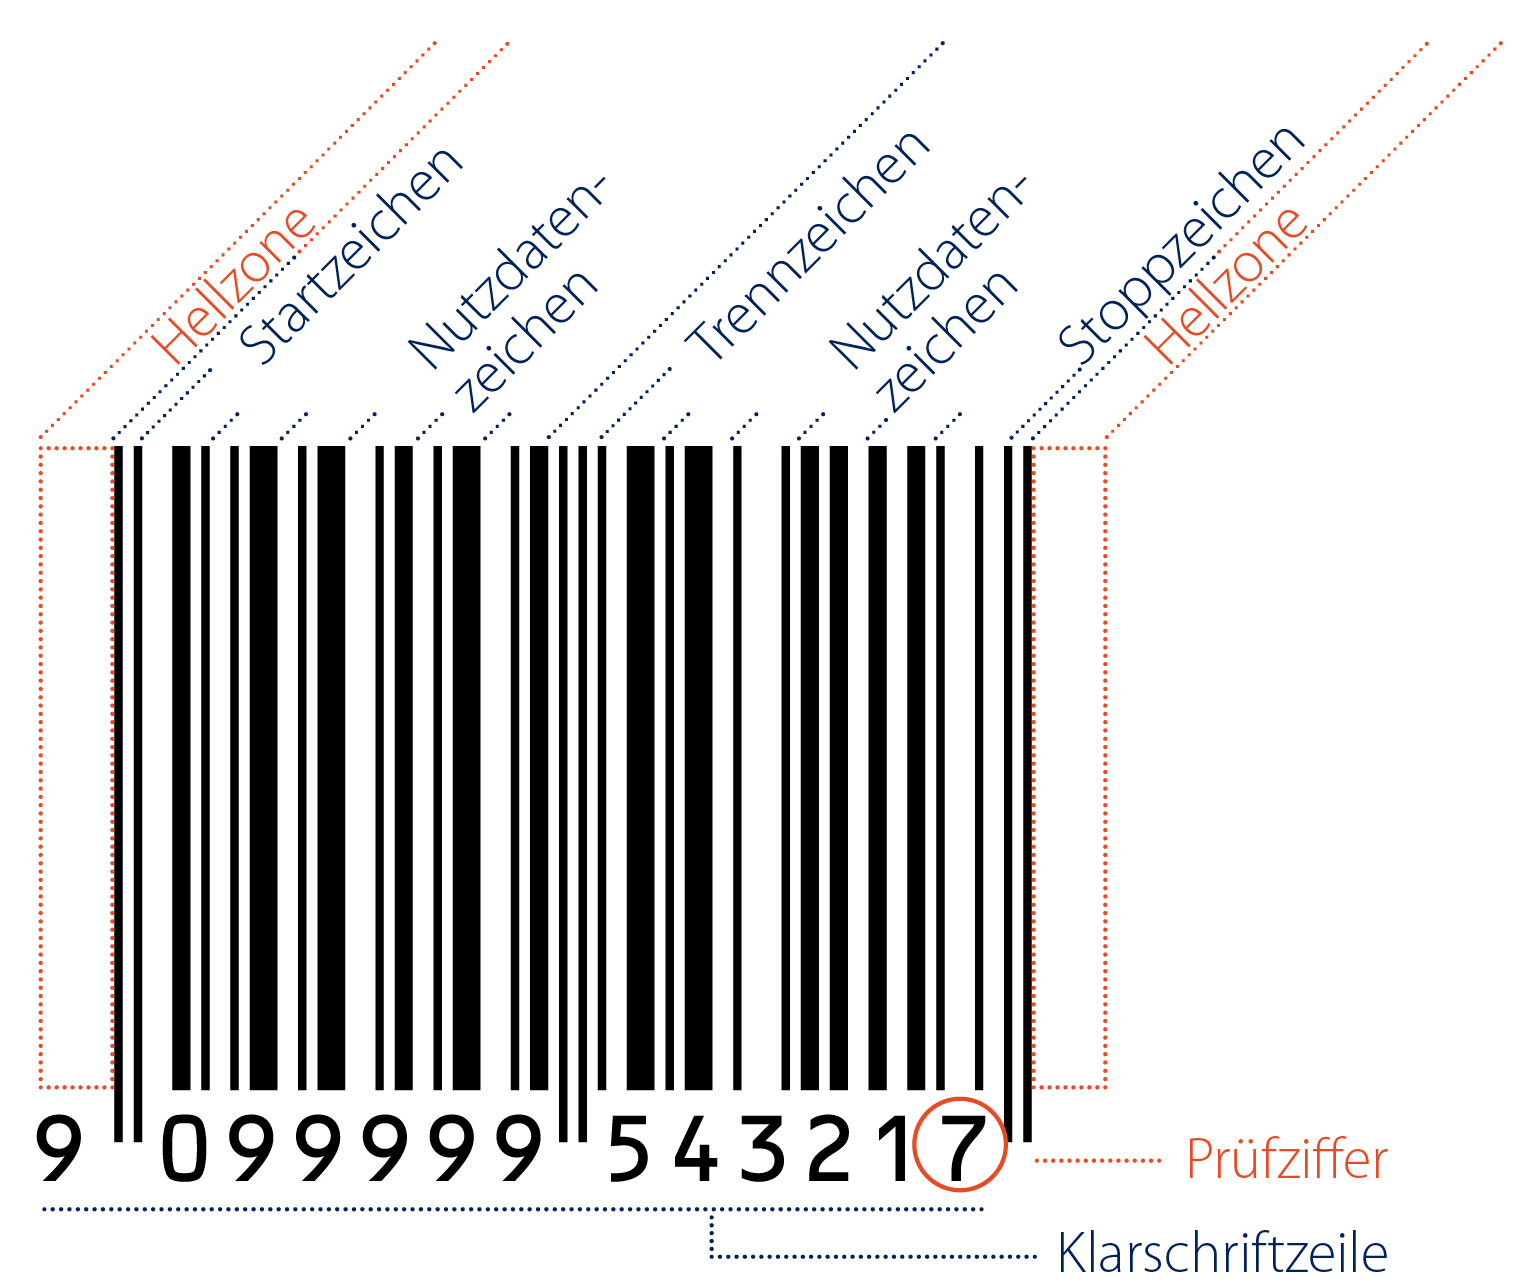
\includegraphics[width=0.8\textwidth]{barcode/ean13barcode.png}
	\caption{EAN-13 Barcode for Organic Oatmeal Cookies}
	\label{fig:ean13_barcode}
\end{figure}

\subsubsection{Barcode Data}

The barcode encodes the following information:

\begin{itemize}
	\item \textbf{Manufacturer Code:} 12345 (Example manufacturer code)
	\item \textbf{Product Code:} 67890 (Example product code)
	\item \textbf{Check Digit:} 5 (Automatically calculated based on manufacturer and product codes)
\end{itemize}

\subsubsection{Usage}

The barcode facilitates the automatic identification and tracking of the ``Organic Oatmeal Cookies'' throughout the supply chain, from manufacturing to retail. It allows for efficient inventory management, accurate pricing, and streamlined checkout processes.

\subsubsection{Labeling}
The barcode is printed on the packaging label of the ``Organic Oatmeal Cookies'' in compliance with regulatory standards. It is placed in a prominent position for easy scanning by retail barcode scanners.




\section{2D Codes: Basic Information}
\subsection{Characteristics of 2D Codes}
\begin{itemize}
	\item \textbf{Large Data Capacity}: Barcodes store data in a single direction, while 2D codes store data in both horizontal and vertical directions, enabling them to hold significantly more information. Standard barcodes can contain up to 30 characters, whereas 2D codes can hold up to 3000 characters.
	
	\item \textbf{High Data Density (Space-Saving)}:2D codes occupy only 1/30 of the space compared to barcodes containing the same amount of data. This compact size allows 2D codes to be attached to electronic components and other small parts where space is limited.
	\item \textbf{Error Correction/Data Recovery}:2D codes feature built-in error correction, enabling data recovery even if the code is damaged or soiled. This is accomplished using mathematical error correction, specifically the Reed-Solomon algorithm.\cite{2Dcodes2024}
\end{itemize}

\textbf{Disadvantages of 2D Codes}
\begin{itemize}
	\item 2D codes lack a backup mechanism if the data becomes unreadable. In contrast, barcodes typically have readable characters below them, allowing staff to manually enter the data using a keyboard if the barcode is damaged or missing, thus ensuring uninterrupted operation. Due to the large amount of data 2D codes contain, adding readable characters is impractical. If a 2D code is too damaged to be scanned, the data cannot be retrieved, leading to operational interruptions. While it is possible to add readable characters to 2D codes, it is unlikely that staff could manually type in more than 100 characters.
\end{itemize}

\subsection{Different Types of 2D Codes}
2D codes are divided into two types based on their structure:
\begin{itemize}
	\item \textbf{Stacked Type}: Conventional barcodes are stacked vertically.
	\item \textbf{Matrix Type}: The data consists of black and white modules in a complex pattern.
\end{itemize}

\subsection{Applications of 2D Codes}
\begin{itemize}
	\item \textbf{Control of Small Parts}: Data Matrix, QR Code, and Veri Code are typical examples of matrix 2D codes. Small parts in industries such as LCD, electronics, semiconductors, and automotive often require several dozen characters to track production history. Since the data needs to be compact to fit on these small parts, matrix 2D codes are commonly used.
	\item \textbf{Shipping Notification, Billing, and Product Labeling with EDI Data}: QR Code, PDF417 (typical). If no database or additional information is available for an item, a 2D code can offer valuable information for product identification.
	\item \textbf{Government Use}: PDF417 (typical). 2D codes are frequently used by governments as a measure against counterfeiting. In Japan, PDF417 codes were used for tickets to the Nagano Olympics. In the USA, 2D codes are commonly found on driver's licenses and ID cards, as they can securely encode portrait images and other critical information.
	\item \textbf{Sorting or Tracking Shipments}: QR Code, Maxi Code (typical). 2D codes are used for automatic high-speed sorting or tracking of shipments in distribution systems.
	\item \textbf{Medical Use}: PDF417 (typical). The "Directive for the New Coding of Prescription Drugs" mandates that certain bio-based products and injectable drugs must include detailed information such as product codes, expiration dates, production numbers, and quantities.
\end{itemize}


\subsection{Structure of QR Codes}
The QR Code (Quick Response Code) is a matrix 2D code designed for high-speed reading, developed by DENSO WAVE in 1994. It was recognized as an AIMI ITS standard in 1997 and as an ISO/IEC standard in 2000. Additionally, the Micro QR Code was standardized as JIS-X-0510 in 2004.

\begin{itemize}
	\item The smallest element of a QR code, whether black or white, is called a "module." A QR code consists of a combination of black and white modules, position detection patterns, timing patterns, format information containing the error correction level and masking numbers, data areas, and an error correction code (Reed-Solomon code).
	\item \textbf{Position Detection Patterns}: These patterns are arranged in three corners of the QR code (and in one corner for Micro QR). The position detection patterns enable the QR code's position to be recognized, facilitating high-speed reading.
	\item \textbf{Alignment Patterns}: The alignment pattern is used for position detection when there is a shift due to distortion. This is applied in Model 2.
	\item \textbf{Margin}: The margin is a blank area around the QR code. Model 1 and 2 require a margin of four modules, and the Micro QR Code requires a margin of two modules.
	\item \textbf{Timing Patterns}: White and black modules are alternately arranged to determine the coordinate.
	\item \textbf{Format Information}: Contains the error correction ratio and the masking pattern of the code. The format information is read first when the code is decoded.
	\item \textbf{Error Correction Code (Reed-Solomon Code)}: The Reed-Solomon code is applied to recover data if the QR code is partially missing or damaged. The recovery ratio varies across four different error correction levels.
\end{itemize}

\subsection{Details of QR Codes}
QR codes are divided into Model 1, Model 2, and Micro QR, each with distinct characteristics and data capacities. The "version" of a QR code indicates its size, measured by the number of modules. Larger versions can contain more data, resulting in an increase in the actual size of the code.

\begin{itemize}
	\item \textbf{Model 1}: Model 1 is the prototype of Model 2 and Micro QR. 1 to 14 versions are standardized by AIMI.
	\item \textbf{Model 2}: Model 2 has an alignment pattern for better positioning and contains more data than Model 1. 1 to 40 versions are standardized by AIMI. Version 40 can hold up to 7089 numeric characters.
	\item \textbf{Micro QR}: The Micro QR Code has only one position detection pattern to reduce size, allowing it to be applied to tiny parts such as printed circuits. The smallest number of modules is 11 × 11. Micro QR codes offer a space-saving alternative.
\end{itemize}

\subsection{Comparison of QR Code Versions}

\begin{longtable}{|m{3.5cm}|m{5cm}|m{6cm}|}
	\hline
	\textbf{Version} & \textbf{Data Capacity (Numeric)} & \textbf{Data Capacity (Alphanumeric)} \\
	\hline
	Model 1 Version 1 & 21 × 21 modules & 10 \\
	\hline
	Model 1 Version 2 & 25 × 25 modules & 20 \\
	\hline
	Model 1 Version 3 & 29 × 29 modules & 35 \\
	\hline
	Model 1 Version 4 & 33 × 33 modules & 50 \\
	\hline
	Model 2 Version 1 & 21 × 21 modules & 41 \\
	\hline
	Model 2 Version 2 & 25 × 25 modules & 77 \\
	\hline
	Model 2 Version 3 & 29 × 29 modules & 127 \\
	\hline
	Model 2 Version 4 & 33 × 33 modules & 187 \\
	\hline
	Model 2 Version 40 & 177 × 177 modules & 7089 \\
	\hline
	Micro QR M1 & 11 × 11 modules & 5 \\
	\hline
	Micro QR M2 & 13 × 13 modules & 10 \\
	\hline
	Micro QR M3 & 15 × 15 modules & 23 \\
	\hline
	Micro QR M4 & 17 × 17 modules & 35 \\
	\hline
	\caption{Comparison of QR Code Versions}
\end{longtable}






%%%%%%%%%%%%%%%%%%

\section{Description}

A strong tool for creating barcodes inside Python programs is the Python Barcode library. It is adaptable for usage in a range of industries, including retail, logistics, and healthcare. It supports a number of barcode formats, including EAN-13, UPC-A, Code 39, and Code 128. Developers can produce high-quality barcodes with little code thanks to the library, which streamlines the barcode generating process.

Generating a barcode is straightforward. Here’s a small example demonstrating how to create an EAN-13 barcode and save it as an image file:
\begin{lstlisting}[caption=Generating and Saving an EAN-13 Barcode]
	import barcode
	from barcode.writer import ImageWriter
	
	# Generate EAN-13 barcode
	ean = barcode.get('ean13', '123456789102', writer=ImageWriter())
	# Save barcode as PNG file
	filename = ean.save('ean13_barcode')
\end{lstlisting}

In this example, the barcode.get() function is used to create an EAN-13 barcode. The ImageWriter class is specified to save the barcode as an image file. This simple yet powerful approach allows developers to integrate barcode generation into their applications effortlessly.

The Python Barcode library also supports customization options, allowing users to adjust the size, text, and formatting of the barcode to meet specific requirements. This flexibility is essential for maintaining consistency with branding and ensuring that the barcodes are readable by standard scanners.

\section{Key Features}
The Python Barcode library supports several widely-used barcode formats including:

\begin{enumerate}
	\item \textbf{Wide Range of Supported Barcode Formats}: The Python Barcode library supports numerous barcode formats, including EAN-13, UPC-A, Code 39, Code 128, and more. This broad compatibility makes it suitable for various applications across different industries, from retail and logistics to healthcare and manufacturing.
	
	\item \textbf{Ease of Use and Simple API}: The library is designed to be user-friendly, featuring a straightforward API that allows developers to generate barcodes with minimal code. For example, creating an EAN-13 barcode involves calling the \texttt{barcode.get()} function and passing the appropriate parameters, making the process quick and efficient.\cite{Barrera:2020}
	
	\item \textbf{Multiple Output Formats}: The library supports exporting barcodes in several formats, such as PNG, SVG, and PDF. This flexibility ensures that developers can use the generated barcodes in different contexts, whether for web applications, printed materials, or digital documents.
	
	\item \textbf{Customization Options}: Developers can easily customize the appearance of barcodes by adjusting parameters like module width, height, font size, text distance, and colors. This feature is essential for maintaining brand consistency and adhering to specific design requirements.
\end{enumerate}

\subsection{Architecture}

The main parts of a Python barcode library's architecture are Barcode Types, Encoder, Decoder, and Utilities. The Barcode Types module defines a number of formats with unique encoding rules, including EAN, UPC, Code 39, Code 128 and QR codes. The encoder converts input data into a barcode image while producing the picture, confirming the data, and adjusting errors. By identifying the barcode, interpreting the patterns, and preparing the image, the Decoder converts barcode images back into data. Utility modules ensure the full functionality of the library by providing support for image handling, checksum calculations, and user interface elements.\\

Validating user input, encoding data into barcode patterns, creating the barcode image, and decoding the image back into data are all steps in the workflow of the library. With methods for creating and decoding barcodes, setting parameters, and managing errors, a well-designed API makes it simple to integrate barcode functionality into applications. A modular architecture and abstract base classes provide extensibility, enabling the addition of new barcode formats and the modification of preexisting ones. This structure is a useful tool for a variety of barcode applications since it guarantees resilience, efficiency, and ease of integration.\cite{Eicebluebarcodepython:2024}\\

\section{Installation}


Installing a Python barcode library involves several steps to ensure that the library is properly integrated and functional within your Python environment. This guide provides a comprehensive overview of the installation process, covering prerequisites, installation steps, and post-installation configuration.

Before installing a barcode library, ensure that system meets the following requirements:

\begin{itemize}
	\item \textbf{Python Installation}: Verify that Python is installed on the system. The library typically supports Python 3.x versions. Check the Python version by running:
	\begin{lstlisting}[language=bash]
		python --version
	\end{lstlisting}
	\item \textbf{PIP}: Ensure that \texttt{pip}, the Python package installer, is installed.Check this by running:
	\begin{lstlisting}[language=bash]
		pip --version
	\end{lstlisting}
\end{itemize}


\subsection*{Installation Steps}

\begin{enumerate}
	\item \textbf{Choose the Barcode Library}: There are several barcode libraries available, such as \texttt{python-barcode} and \texttt{qrcode}. This guide focuses on installing \texttt{python-barcode}.
	
	\item \textbf{Install the Library}: Use \texttt{pip} to install the \texttt{python-barcode} library. Open your terminal or command prompt and run:
	\begin{lstlisting}[language=bash]
		pip install python-barcode
	\end{lstlisting}
	
	\item \textbf{Install Additional Dependencies}: Some barcode libraries require additional dependencies for generating and handling images. For \texttt{python-barcode},might need the \texttt{Pillow} library for image processing. Install it using:
	\begin{lstlisting}[language=bash]
		pip install pillow
	\end{lstlisting}
\end{enumerate}

\subsection*{Post-Installation Configuration}

\begin{enumerate}
	\item \textbf{Verify Installation}: After installation, verify that the library and its dependencies are correctly installed. We can do this by opening a Python interpreter and importing the library:
	\begin{lstlisting}[language=Python]
		import barcode
		from barcode.writer import ImageWriter
	\end{lstlisting}
	
	\item \textbf{Testing Basic Functionality}: Create a simple script to generate a barcode to ensure everything is working correctly. Save the following code in a file named \texttt{barcode\_test.py}:
	\begin{lstlisting}[language=Python]
		import barcode
		from barcode.writer import ImageWriter
		
		# Choose the barcode format
		EAN = barcode.get_barcode_class('ean13')
		
		# Provide the data for the barcode
		ean = EAN('123456789102', writer=ImageWriter())
		
		# Save the barcode as an image file
		filename = ean.save('ean13_barcode')
		print(f'Barcode saved as {filename}.png')
	\end{lstlisting}
	
	Run the script:
	\begin{lstlisting}[language=bash]
		python barcode_test.py
	\end{lstlisting}
	
	This script should generate an EAN-13 barcode and save it as an image file named \texttt{ean13\_barcode.png}.
	
	\item \textbf{Explore Documentation}: Familiarize with the library's documentation to understand the various functionalities and customization options available. The documentation often provides examples and detailed explanations of the library's features.
\end{enumerate}


\subsection*{Troubleshooting}

\begin{itemize}
	\item \textbf{Dependency Issues}: If we encounter issues related to missing dependencies, ensure all required packages are installed. Use \texttt{pip list} to check installed packages and their versions.
	
	\item \textbf{Environment Configuration}: For advanced usage, consider setting up a virtual environment to manage dependencies and avoid conflicts. Create a virtual environment with:
	\begin{lstlisting}[language=bash]
		python -m venv barcode_env
		source barcode_env/bin/activate  # On Windows use `barcode_env\Scripts\activate`
	\end{lstlisting}
	
\end{itemize}

\section{Example - Generating Barcodes}

Generating barcodes is a critical task in various applications, ranging from retail to logistics. A Python barcode library simplifies this process by providing robust tools for creating barcodes in multiple formats. 

\subsection{3.1 Supported Barcode Formats}

A Python barcode library typically supports a variety of barcode formats to cater to different industry needs. Here is a list of common barcode formats supported by most libraries, along with their descriptions and use cases:\\

\subsubsection{EAN-13 (European Article Number)}

EAN-13 is a 13-digit barcode widely used in global retail for product identification. It encodes a product's unique identifier, facilitating inventory management and point-of-sale transactions. EAN-13 consists of a country code, manufacturer code, product code, and a checksum digit. It is prevalent in supermarkets and retail stores.\cite{Barrera:2020}

\subsubsection{UPC-A (Universal Product Code)}

UPC-A is a 12-digit barcode primarily used in North America for similar purposes as EAN-13. It encodes a numeric identifier that includes a manufacturer number and an item number, along with a check digit. UPC-A is integral to the retail industry, enabling efficient tracking and checkout processes.

\subsubsection{Code 39}

Code 39, also known as Code 3 of 9, is an alphanumeric barcode that can encode both letters and numbers. It is widely used in various industries, including automotive and defense, due to its versatility and simplicity. Each character in Code 39 is represented by nine elements: five bars and four spaces. It is often used for inventory labeling and tracking.

\subsubsection{Code 128}

Code 128 is a high-density barcode capable of encoding all 128 ASCII characters. It is used in logistics and transportation for encoding complex data such as shipment information, serial numbers, and product codes. Code 128 offers excellent data security and is efficient in terms of space, making it suitable for a wide range of applications.

\subsubsection{QR Code (Quick Response Code)}

QR Code is a two-dimensional barcode that can store a large amount of data, including numeric, alphanumeric, binary, and Kanji characters. QR Codes are widely used in various applications such as marketing, ticketing, and product tracking. Their ability to be scanned by smartphones has made them popular in modern digital interactions.\cite{Barrera:2020}

\subsection{Generating Barcodes}

To generate barcodes, follow these steps using a Python barcode library:

\begin{enumerate}
	\item \textbf{Choose the Barcode Format}: Select the appropriate format based on the application's requirements.
	\item \textbf{Install the Library}: Ensure the barcode library and its dependencies are installed.
	\item \textbf{Encode Data}: Use the library to encode the required data into the selected barcode format.
	\item \textbf{Save the Barcode}: Generate the barcode image and save it in the desired format (e.g., PNG, SVG).
\end{enumerate}

Here is an example of generating an EAN-13 barcode using the \texttt{python-barcode} library:

\begin{lstlisting}[language=Python]
	import barcode
	from barcode.writer import ImageWriter
	
	# Choose the barcode format
	EAN = barcode.get_barcode_class('ean13')
	
	# Provide the data for the barcode
	ean = EAN('123456789102', writer=ImageWriter())
	
	# Save the barcode as an image file
	filename = ean.save('ean13_barcode')
	print(f'Barcode saved as {filename}.png')
\end{lstlisting}

This example demonstrates the simplicity and effectiveness of generating barcodes using a Python library. By understanding and leveraging these barcode formats, developers can efficiently integrate barcode functionalities into their applications, enhancing automation and data management capabilities.

\section{Example - Basic Concepts of Python Barcode}

Generating barcodes with a Python barcode library is a straightforward process that involves initializing the library, selecting the barcode type, and generating the barcode image.

Generating Different Types of Barcodes\\

The \texttt{python-barcode} library supports multiple barcode formats. Here are some examples of generating different barcode types: \cite{Barrera:2020}

\begin{itemize}
	\item \textbf{Code 39}:
	\begin{lstlisting}[language=Python]
		CODE39 = barcode.get_barcode_class('code39')
		code39 = CODE39('HELLO123', writer=ImageWriter())
		filename = code39.save('code39_barcode')
		print(f'Barcode saved as {filename}.png')
	\end{lstlisting}
	
	\item \textbf{UPC-A}:
	\begin{lstlisting}[language=Python]
		UPCA = barcode.get_barcode_class('upca')
		upca = UPCA('123456789102', writer=ImageWriter())
		filename = upca.save('upca_barcode')
		print(f'Barcode saved as {filename}.png')
	\end{lstlisting}
\end{itemize}

\subsection{Customizing Barcodes}

Customizing the appearance of barcodes can be crucial for ensuring they meet specific requirements or aesthetic preferences. The \texttt{python-barcode} library allows customization of various properties such as size, text, and font.

\subsubsection{Customizing Barcode Properties}

\begin{itemize}
	\item \textbf{Size Customization}:
	You can customize the size of the barcode by adjusting the writer's parameters.
	\begin{lstlisting}[language=Python]
		options = {
			'module_width': 0.2,
			'module_height': 15.0,
			'quiet_zone': 6.5,
			'font_size': 10,
			'text_distance': 5.0,
			'background': 'white',
			'foreground': 'black',
			'write_text': True,
		}
		
		ean = EAN('123456789102', writer=ImageWriter())
		filename = ean.save('custom_ean13_barcode', options=options)
		print(f'Barcode saved as {filename}.png')
	\end{lstlisting}
	
	\item \textbf{Text and Font Customization}:
	To customize the text and font properties of the barcode, modify the \texttt{options} dictionary.
	\begin{lstlisting}[language=Python]
		options = {
			'font_size': 18,        # Increase the font size
			'text_distance': 3,     # Reduce the distance between the barcode and text
		}
		
		ean = EAN('123456789102', writer=ImageWriter())
		filename = ean.save('text_custom_ean13_barcode', options=options)
		print(f'Barcode saved as {filename}.png')
	\end{lstlisting}
	
	\item \textbf{Color Customization}:
	Adjust the foreground and background colors of the barcode to match specific design requirements.\cite{Oliverpython:2023}
	\begin{lstlisting}[language=Python]
		options = {
			'background': 'yellow',   # Set the background color to yellow
			'foreground': 'blue',     # Set the barcode color to blue
		}
		
		ean = EAN('123456789102', writer=ImageWriter())
		filename = ean.save('color_custom_ean13_barcode', options=options)
		print(f'Barcode saved as {filename}.png')
	\end{lstlisting}
\end{itemize}

\subsubsection{Customizing QR Code Appearance}

The \texttt{qrcode} package allows extensive customization of QR code aesthetics, enabling you to tailor the design to specific requirements. Key customization options include:

\begin{itemize}
	\item \textbf{Box Size}: Defines the number of pixels for each box in the QR code matrix.
	\item \textbf{Border}: Sets the thickness of the border (measured in boxes) surrounding the QR code.
	\item \textbf{Fill and Background Colors}: Allows setting the colors of the QR code and its background, supporting various color schemes beyond the default black-and-white.
\end{itemize}

\bigskip

\textbf{Example}:

\begin{lstlisting}[language=Python]
	import qrcode
	
	# Create a QR code instance with custom settings
	qr = qrcode.QRCode(
	version=1,
	error_correction=qrcode.constants.ERROR_CORRECT_L,
	box_size=10,
	border=4,
	)
	
	# Add data to the QR code
	qr.add_data('https://www.example.com')
	qr.make(fit=True)
	
	# Generate the image with custom colors
	img = qr.make_image(fill_color="blue", back_color="white")
	img.save('custom_qr.png')
\end{lstlisting}

\begin{center}
	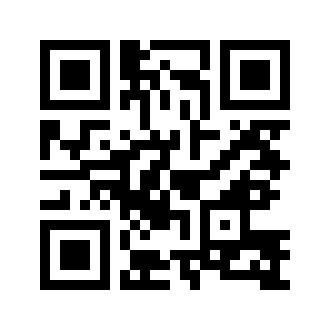
\includegraphics[width=0.5\textwidth]{PythonBarcode/qrcode3}
	\captionof{figure}{Customizing QR Code}\label{Customizing QR Code}
\end{center}

In this example, the QR code is generated with a blue fill color and a white background, demonstrating the package's flexibility in design customization.\cite{geeksforgeeksqrcode:2023}

\subsection{Embedding Logos or Images}

Enhancing QR codes by embedding logos or images can improve brand recognition and aesthetics. This can be achieved by combining the \texttt{qrcode} package with the \texttt{Pillow} package, which facilitates image manipulation.

\textbf{Example}:
\begin{lstlisting}[language=Python]
	import qrcode
	from PIL import Image
	
	# Generate the QR code
	qr = qrcode.QRCode(
	error_correction=qrcode.constants.ERROR_CORRECT_H
	)
	qr.add_data('https://www.example.com')
	qr.make(fit=True)
	img = qr.make_image(fill_color="black", back_color="white").convert('RGB')
	
	# Open the logo image
	logo = Image.open('logo.png')
	
	# Calculate dimensions for the logo
	box = (img.size[0] // 2 - logo.size[0] // 2,
	img.size[1] // 2 - logo.size[1] // 2,
	img.size[0] // 2 + logo.size[0] // 2,
	img.size[1] // 2 + logo.size[1] // 2)
	
	# Paste the logo onto the QR code
	img.paste(logo, box, mask=logo)
	img.save('qr_with_logo.png')
\end{lstlisting}

This script generates a QR code and embeds a logo at its center, creating a branded QR code. The \texttt{error\_correction} parameter is set to \texttt{ERROR\_CORRECT\_H} to ensure the QR code remains scannable despite the embedded image.

\subsection{Generating QR Codes for Various Data Types}

The \texttt{qrcode} package supports encoding different data types, including URLs, text, contact information, and Wi-Fi credentials. This versatility makes it suitable for a wide range of applications.

\textbf{Example}:
\begin{lstlisting}[language=Python]
	import qrcode
	
	# Wi-Fi credentials
	wifi_ssid = 'YourSSID'
	wifi_password = 'YourPassword'
	wifi_type = 'WPA'  # or 'WEP'
	
	# Create Wi-Fi QR code data string
	wifi_data = f'WIFI:S:{wifi_ssid};T:{wifi_type};P:{wifi_password};;'
	
	# Generate the QR code
	qr = qrcode.make(wifi_data)
	qr.save('wifi_qr.png')
\end{lstlisting}

This example generates a QR code containing Wi-Fi credentials, allowing users to connect to the network by scanning the code.\cite{geeksforgeeksqrcode:2023}

\subsection{Batch Processing for Multiple QR Codes}

When dealing with large datasets, the \texttt{qrcode} package facilitates batch processing, enabling the generation of multiple QR codes efficiently.

\textbf{Example}:
\begin{lstlisting}[language=Python]
	import qrcode
	
	# List of URLs to encode
	urls = [
	'https://www.example.com/page1',
	'https://www.example.com/page2',
	'https://www.example.com/page3',
	]
	
	# Generate QR codes for each URL
	for idx, url in enumerate(urls, start=1):
	qr = qrcode.make(url)
	qr.save(f'qr_code_{idx}.png')
\end{lstlisting}

This script iterates over a list of URLs, generating and saving a QR code for each, demonstrating the package's capability to handle batch operations effectively.

\subsection{Error Correction Levels}

The \texttt{qrcode} package supports different error correction levels, which determine the QR code's resilience to damage or obscuration. Higher error correction levels allow the QR code to be read even if a portion is missing or unreadable. The available levels are:

\begin{itemize}
	\item \textbf{L}: Approximately 7\% error correction
	\item \textbf{M}: Approximately 15\% error correction
	\item \textbf{Q}: Approximately 25\% error correction
	\item \textbf{H}: Approximately 30\% error correction
\end{itemize}

\textbf{Example}:
\begin{lstlisting}[language=Python]
	import qrcode
	
	# Create a QR code with high error correction
	qr = qrcode.QRCode(
	error_correction=qrcode.constants.ERROR_CORRECT_H
	)
	qr.add_data('https://www.example.com')
	qr.make(fit=True)
	img = qr.make_image(fill_color="black", back_color="white")
	img.save('high_error_correction_qr.png')
\end{lstlisting}

In this example, the QR code is generated with the highest error correction level (\texttt{ERROR\_CORRECT\_H}), ensuring it remains scannable even if up to 30\% of the code is damaged or obscured.

By leveraging these advanced features, the Python \texttt{qrcode} package provides a robust solution for generating customized, resilient, and versatile QR codes suitable for various applications. \cite{geeksforgeeksqrcode:2023}

\subsection{Saving and Exporting Barcodes}

Exporting and storing barcodes to various file formats is an essential function of a Python barcode library. This section examines the benefits of the many available file formats and offers sample code snippets for barcodes saved in each format.\cite{Zellepython:2004}

\subsubsection{Saving to Different File Formats}

Barcode libraries typically support multiple file formats to cater to diverse needs. Common formats include PNG, SVG, and PDF, each with distinct advantages:

\begin{itemize}
	\item \textbf{PNG}: A raster graphics format that is widely supported and suitable for web use.
	\item \textbf{SVG}: A vector graphics format that allows for scalability without loss of quality, ideal for print and high-resolution displays.
	\item \textbf{PDF}: A document format that supports embedding of barcodes in documents, useful for reports and printable materials.
\end{itemize}

Saving barcodes as PDFs can be useful for creating documents that include barcode images.

\begin{lstlisting}
	import barcode
	from barcode.writer import ImageWriter
	
	# Choose the barcode format
	EAN = barcode.get_barcode_class('ean13')
	
	# Provide the data for the barcode
	ean = EAN('123456789102', writer=ImageWriter())
	
	# Save the barcode as a PDF file
	filename = ean.save('ean13_barcode', options={"write_text": False})
	print(f'Barcode saved as {filename}.pdf')
\end{lstlisting}

The Python barcode library may be made more functional by integrating it with other libraries, and thus gives developers a strong toolkit for creating complete barcode solutions. One of the most popular integrations is with the sophisticated image editing capabilities of the Python Imaging Library (PIL), which is now called Pillow. This section explains how to integrate the Python barcode library with Pillow in an efficient manner and offers useful code examples to show how to do so.\\

\subsubsection{Using the Python Barcode Library with Pillow}

Pillow is a powerful image processing library in Python, which adds image manipulation capabilities such as resizing, cropping, filtering, and format conversion. By integrating the barcode library with Pillow, we can customize and manipulate barcode images to fit specific requirements.

\subsection{Example Code Demonstrating Integration}

Below is an example of how to generate a barcode using the \texttt{python-barcode} library and manipulate it using Pillow:

\subsubsection{Install the Necessary Libraries}

Ensure both \texttt{python-barcode} and \texttt{Pillow} are installed:
\begin{lstlisting}[language=bash]
	pip install python-barcode pillow
\end{lstlisting}

\subsubsection{Generate a Barcode and Manipulate with Pillow}

The following code demonstrates generating an EAN-13 barcode, converting it to a Pillow image object, and then performing some basic image manipulations:
\begin{lstlisting}[language=Python]
	import barcode
	from barcode.writer import ImageWriter
	from PIL import Image, ImageEnhance, ImageFilter
	
	# Generate the barcode
	EAN = barcode.get_barcode_class('ean13')
	ean = EAN('123456789102', writer=ImageWriter())
	
	# Save the barcode as an image file
	barcode_filename = ean.save('ean13_barcode')
	
	# Open the barcode image with Pillow
	barcode_image = Image.open(f"{barcode_filename}.png")
	
	# Enhance the image
	enhancer = ImageEnhance.Contrast(barcode_image)
	enhanced_image = enhancer.enhance(2.0)  # Increase contrast
	
	# Apply a filter to the image
	filtered_image = enhanced_image.filter(ImageFilter.SHARPEN)
	
	# Save the modified image
	filtered_image.save('enhanced_ean13_barcode.png')
	
	# Display the image (optional, for testing purposes)
	filtered_image.show()
\end{lstlisting}

\subsubsection{Explanation of the Code}

\begin{itemize}
	\item \textbf{Barcode Generation}: The code generates an EAN-13 barcode using the \texttt{python-barcode} library and saves it as an image file.
	\item \textbf{Image Opening}: The generated barcode image is opened using Pillow, converting it into an \texttt{Image} object.
	\item \textbf{Image Enhancement}: The contrast of the image is enhanced using \texttt{ImageEnhance.Contrast}.
	\item \textbf{Image Filtering}: A sharpening filter is applied to the image using \texttt{ImageFilter.SHARPEN}.
	\item \textbf{Saving the Image}: The modified image is saved to a new file.
	\item \textbf{Displaying the Image}: The final image can be displayed on the screen for verification (optional).
\end{itemize}

\subsection{Reading and Decoding Barcodes}

Reading and decoding barcodes in Python can be efficiently achieved using several libraries, each offering unique features and advantages. Two of the most commonly used libraries are \textbf{pyzbar} and \textbf{OpenCV}.\\

\textbf{Pyzbar} is a lightweight and easy-to-use library specifically designed for barcode and QR code decoding. It supports a wide range of barcode formats, including EAN, UPC, Code 128, and QR codes. Pyzbar is particularly useful in applications where simplicity and quick integration are key, as it requires minimal setup and has a straightforward API.\\

\textbf{OpenCV} (Open Source Computer Vision Library) is a more comprehensive library that provides extensive tools for image processing and computer vision tasks. While OpenCV is not specifically designed for barcode decoding, it includes functionalities for detecting and interpreting barcodes through image processing techniques. OpenCV is particularly suitable for complex applications that require advanced image manipulation, such as adjusting contrast, thresholding, or working with multiple barcode formats in challenging environments.\\


\subsection{Implementing Barcode Reading}
\subsubsection{Using Pyzbar}

\begin{lstlisting}
	from pyzbar.pyzbar import decode
	from PIL import Image
	
	# Load the image
	image = Image.open('barcode.png')
	
	# Decode the barcode
	barcodes = decode(image)
	
	for barcode in barcodes:
	barcode_data = barcode.data.decode('utf-8')
	barcode_type = barcode.type
	print(f'Found {barcode_type} barcode: {barcode_data}')
\end{lstlisting}

This code loads an image containing a barcode, decodes it using Pyzbar, and prints the barcode type and data.

\subsubsection{Using OpenCV}

\begin{lstlisting}
	import cv2
	from pyzbar.pyzbar import decode
	
	# Load the image
	image = cv2.imread('barcode.png')
	
	# Convert to grayscale (optional)
	gray_image = cv2.cvtColor(image, cv2.COLOR_BGR2GRAY)
	
	# Decode the barcode
	barcodes = decode(gray_image)
	
	for barcode in barcodes:
	barcode_data = barcode.data.decode('utf-8')
	barcode_type = barcode.type
	print(f'Found {barcode_type} barcode: {barcode_data}')
\end{lstlisting}

This example uses OpenCV to load and optionally preprocess the image by converting it to grayscale before decoding it with Pyzbar. Grayscale conversion can improve accuracy in some cases, particularly with noisy images.


\section{Example - Advanced Features: Batch Processing in Python Barcode Library}

\subsection{Overview of Batch Processing}

Batch processing in a Python barcode library refers to the generation of multiple barcodes in a single operation. This feature is particularly useful in scenarios where a large number of barcodes need to be created at once, such as in inventory management, product labeling, or shipping operations. By leveraging batch processing, developers can streamline the process of barcode generation, reducing the overhead associated with generating each barcode individually.

\subsection{Generating Multiple Barcodes in Batch Mode}

Batch processing involves reading a dataset containing multiple items, each with its associated data to be encoded into a barcode. The Python barcode library typically allows this data to be read from various sources, such as CSV files, databases, or lists within a script. The key steps in batch processing are:

\begin{enumerate}
	\item \textbf{Data Input}: Collect or load the dataset that contains the information for each barcode.
	\item \textbf{Barcode Generation}: Iterate over the dataset, generating a barcode for each item.
	\item \textbf{File Handling}: Optionally, save each barcode to a file or handle them in-memory for further processing.
\end{enumerate}

\subsubsection{Example Code for Batch Barcode Generation}

Below is a Python script that demonstrates how to implement batch barcode generation using the \texttt{python-barcode} library. The script reads product data from a CSV file and generates an EAN-13 barcode for each product.

\begin{lstlisting}[language=Python]
	import csv
	import barcode
	from barcode.writer import ImageWriter
	
	# Function to generate barcodes in batch mode
	def generate_barcodes(csv_file, output_dir):
	with open(csv_file, newline='') as file:
	reader = csv.DictReader(file)
	for row in reader:
	# Extract product code and name from each row
	product_code = row['product_code']
	product_name = row['product_name']
	
	# Generate an EAN-13 barcode
	EAN = barcode.get_barcode_class('ean13')
	ean = EAN(product_code, writer=ImageWriter())
	
	# Save the barcode as an image file in the specified output directory
	file_path = f"{output_dir}/{product_name}_barcode.png"
	ean.save(file_path)
	print(f"Generated barcode for {product_name} saved as {file_path}")
	
	# Example usage
	csv_file = 'products.csv'
	output_dir = 'barcodes'
	generate_barcodes(csv_file, output_dir)
\end{lstlisting}



\section{Error Handling and Validation in Python Barcode Library}

When working with a Python barcode library, proper error handling and data validation are crucial to ensuring that the barcodes generated are accurate and usable. This section discusses common errors encountered during barcode generation, how to handle them, and best practices for validating barcode data before generation.

\subsection{Common Errors and Their Handling}


A common error occurs when the input data does not conform to the expected format for the chosen barcode type. For instance, an EAN-13 barcode requires a 12-digit numeric input, but if the user provides alphanumeric characters or an incorrect length, an exception will be raised. To handle this, you should validate the input data before attempting to generate the barcode.

\textbf{Handling}:
\begin{lstlisting}[language=Python]
	try:
	ean = EAN('1234567ABC12', writer=ImageWriter())
	except ValueError as e:
	print(f"Error: {e}. Please provide a 12-digit numeric input.")
\end{lstlisting}



\subsubsection{Missing Dependencies}
Another common issue is missing dependencies, especially when image handling is required. If the \texttt{Pillow} library (used for image processing) is not installed, the barcode generation that requires an image output will fail.

\textbf{Handling}:
Before generating a barcode that requires an image, ensure that the necessary libraries are installed. This can be done programmatically:
\begin{lstlisting}[language=Python]
	try:
	from PIL import Image
	except ImportError:
	raise ImportError("Pillow library is not installed. Please install it using `pip install pillow`.")
\end{lstlisting}



\subsubsection{File I/O Errors}
File input/output errors can occur when saving the generated barcode to a file. These errors might include permission errors, invalid file paths, or disk space issues.

\textbf{Handling}:
\begin{lstlisting}[language=Python]
	try:
	filename = ean.save('/invalid/path/ean13_barcode')
	except OSError as e:
	print(f"Error saving barcode: {e}")
\end{lstlisting}



\subsection{Validating Barcode Data Before Generation}

\subsubsection{Length and Character Set Validation}
Each barcode type has specific requirements regarding the length and character set of the input data. For example, Code 128 supports a wide range of characters, while EAN-13 is limited to 12 digits. Implementing validation checks before generating the barcode helps avoid runtime errors.

\begin{lstlisting}[language=Python]
	def validate_ean13(data):
	if len(data) != 12 or not data.isdigit():
	raise ValueError("EAN-13 barcode requires a 12-digit numeric input.")
\end{lstlisting}

\noindent Before generating an EAN-13 barcode, you can call \texttt{validate\_ean13(data)} to ensure that the input meets the required standards.



\subsubsection{Checksum Verification}
Some barcode formats, like EAN and UPC, include a checksum digit, which is the final digit of the barcode. Verifying the checksum before generating the barcode ensures that the data is valid. Many libraries automatically handle checksum calculation, but it is good practice to understand and verify it manually if necessary.

\begin{lstlisting}[language=Python]
	def calculate_ean13_checksum(data):
	if len(data) != 12:
	raise ValueError("Checksum can only be calculated for 12-digit EAN-13 data.")
	odd_sum = sum(int(data[i]) for i in range(0, 12, 2))
	even_sum = sum(int(data[i]) for i in range(1, 12, 2))
	total_sum = odd_sum + 3 * even_sum
	return (10 - (total_sum % 10)) % 10
\end{lstlisting}

\noindent This function calculates the checksum for EAN-13 data, which can be compared with the provided checksum to validate the data.



\subsubsection{Pre-generation Simulation}
For complex barcode types or large datasets, simulating barcode generation without creating files can help identify issues early. This technique involves running the data through the encoding process and catching any errors that arise, without saving the output.

\begin{lstlisting}[language=Python]
	def simulate_barcode_generation(data, barcode_type):
	try:
	barcode_instance = barcode_type(data)
	barcode_instance.build()  # Simulate the generation process
	except Exception as e:
	print(f"Simulation failed: {e}")
\end{lstlisting}

\noindent This method helps identify issues like incorrect data or configuration settings before committing to file generation.

\section{Error Handling in Python Barcode}

Error handling in the Python \texttt{barcode} package is essential to ensure smooth code execution and user feedback in cases of invalid input, unsupported formats, or other issues. Common errors in generating barcodes might include providing an incorrect data length for specific barcode types (like EAN-13, which requires 12 digits), using an unsupported barcode format, or encountering file-related issues when saving the generated barcode image. To handle such errors gracefully, \texttt{try-except} blocks are commonly used in Python. For example, wrapping barcode generation code in a \texttt{try-except} block allows developers to catch specific exceptions, such as \texttt{ValueError} for invalid barcode data or \texttt{IOError} for issues when saving the image. By catching these exceptions, custom error messages can inform the user about the specific problem, guiding them on how to correct it.

Advanced error handling also involves validating input data before attempting barcode generation. For example, checking the length of data before passing it to an EAN-13 barcode generation function can prevent unnecessary exceptions, thereby improving the program's reliability. The package may also throw errors when trying to use unsupported formats or writers (such as attempting to save a barcode as an unsupported file type). Additionally, using error handling to manage dependencies (e.g., ensuring \texttt{Pillow} is installed when generating image-based barcodes) can prevent runtime errors. Effective error handling ensures that the program remains robust, providing users with feedback that enhances usability and helps prevent data entry mistakes. \cite{hichembarcode:2023}

\section{Further Resources}

\textit{Python Barcode package Documentation}- Python-Barcode Documentation \cite{Pythonbarcodepackage:2024}:

This official documentation provides a thorough overview of the Python Barcode package, explaining its functionality and how to generate barcodes in various formats, such as EAN, Code39, and Code128. The documentation includes detailed instructions, examples, and customization options for generating and managing barcodes effectively. This resource is valuable for developers looking to integrate barcode functionality into Python applications, with comprehensive examples and usage details.


\textit{Barcode Detection in Image Processing}- A Study on Multiple Barcode Detection from an Image in Business System by Atiqul Islam Chowdhury \cite{Chowdhury:2019}:

This paper explores techniques for detecting multiple barcodes within a single image in business applications. It analyzes various image processing methods that enhance barcode detection accuracy, making it especially useful for inventory management and retail systems. The study discusses challenges and solutions associated with barcode detection in real-world environments and provides insights into handling image noise, lighting variations, and overlapping barcodes.

\textit{Advanced Barcode Generation in Python} - Barcode Generation and Recognition using Python \cite{Ijesat:2023}:

This article, published in the International Journal of Engineering Science and Advanced Technology (IJESAT), provides a technical perspective on barcode generation and recognition using Python. It covers the integration of barcode generation with OpenCV for enhanced image processing, as well as barcode detection techniques in complex images. The article emphasizes Python’s role in efficient barcode handling for business and industrial systems, offering practical code implementations and case studies on barcode recognition and data extraction.
